\chapter{Introduction}

The Jiangmen Underground Neutrino Observatory (JUNO), currently under construction in southern China, is a large liquid scintillator neutrino detector. It is designed to detect electron antineutrino interactions produced by nearby Nuclear Power Plants (NPP) through the inverse beta decay reaction. The primary objective of this experiment is to determine the neutrino mass hierarchy, thereby addressing the Neutrino Mass Ordering (NMO) problem.

The field of neutrino physics has entered a new era of precision following the measurement of the third lepton mixing angle, the so-called reactor angle $\theta_{13}$. This has had a significant impact on models of neutrino mass and mixing. The JUNO experiment, with its excellent energy resolution and large fiducial volume, is expected to make significant contributions to this field.

This leads us to the theory of neutrino oscillation, a quantum mechanical phenomenon whereby a neutrino created with a specific lepton flavor can later be measured to have a different flavor. The oscillation is quantified in terms of parameters that the JUNO experiment aims to measure with high precision.


\section{Neutrinos Oscillation}
The Standard Model of elementary particle interactions provides an accurate description of strong, weak, and electromagnetic interactions, but it treats these interactions as distinct and unrelated. Within this framework, neutrinos are assumed to be massless, but this assumption has been called into question by physicists. Neutrino oscillations, are a potential indication of neutrino mass.\\
The term "neutrino oscillations" refers to this phenomena and it involve the conversion of a neutrino of a particular flavor to another as it propagates through space.

Each known flavor eigenstate, $(\nu_e,\nu_{\mu},\nu_{\tau})$, linked to three respective charged leptons $(e,\mu,\tau)$  via the charged current interactions can be considered a complex combination of neutrino mass eigenstates as follow:

\begin{equation*}
	\left(\begin{array}{l}
		v_e \\
		v_\mu \\
		v_\tau
	\end{array}\right)=U_{\mathrm{PMNS}}\left(\begin{array}{l}
		v_1 \\
		v_2 \\
		v_3
	\end{array}\right)
\end{equation*}
in wich $\nu_i$ are the three mass eigensates, that have 3 masses  $m_i$  $(i = 1,2,3)$, which are non-degenerate, with $m_i \neq m_j$ for $i \neq j$.\\

The matrix $U_{\mathrm{PMNS}}$, called Pontecorvo-Maki-Nakagawa-Sakata (PMNS) matrix, is composed of three rotation matrices, $R_{23}$, $R_{13}$, and $R_{12}$, each corresponding to a different mixing angle, $\theta_{23}$, $\theta_{13}$, and $\theta_{12}$, respectively and a parameter $\delta_{CP}$ called the Dirac CP-violating phase. For this case, the Majorana $C P$ phases are $\eta_i(i=1,2)$, which are only physically possible if neutrinos are Majorana-type particles and do not participate in neutrino oscillations. Therefore, $U$ can be expressed as:

\begin{equation*} 
	\begin{split}
			U_{\text {PMNS }}&=\\
		=&\left(\begin{array}{ccc}
			1 & 0 & 0 \\
			0 & c_{23} & s_{23} \\
			0 & -s_{23} & c_{23}
		\end{array}\right) \left(\begin{array}{ccc}
			c_{13} & 0 & s_{13} \mathrm{e}^{-\mathrm{i} \delta_{C P}} \\
			0 & 1 & 0 \\
			-s_{13} \mathrm{e}^{\mathrm{i} \delta_{C P}} & 0 & c_{13}
		\end{array}\right) 
		\left(\begin{array}{ccc}
			c_{12} & s_{12} & 0 \\
			-s_{12} & c_{12} & 0 \\
			0 & 0 & 1
		\end{array}\right)\left(\begin{array}{ccc}
			\mathrm{e}^{\mathrm{i} \eta_1} & 0 & 0 \\
			0 & \mathrm{e}^{\mathrm{i} \eta_2} & 0 \\
			0 & 0 & 1
		\end{array}\right)
	\end{split}
\end{equation*}
where $s_{i j} \equiv \sin \theta_{i j}, c_{i j} \equiv \cos \theta_{i j}$.

The theoretical framework for neutrino oscillations involves the calculation of the oscillation probability as a function of the distance traveled by the neutrino, the neutrino mixing matrix, and the difference in squared masses between the three neutrino mass states, $\Delta m_{ij}^2 = m^2_i - m^2_j$ for $i,j = 1,2,3, i>j$ . Specifically, two nuclear power reactors 53 $\unit{\kilo\meter}$ away from the detector, which mostly produce anti-electron neutrinos $\bar{\nu}_e$ with energy below 10 MeV, are the principal sources of neutrinos for the JUNO experiment. So, it is necessary for the JUNO experiment to calculate the survival probability $P\left(\bar{\nu}_e \rightarrow \bar{\nu}_e\right)$ of electron antineutrinos.

\begin{equation*}
	P\left(\bar{\nu}_e \rightarrow \bar{\nu}_e\right)=1-\sin ^2 2 \theta_{12} c_{13}^4 \sin ^2\left(\frac{\Delta m_{21}^2 L}{4 \mathcal{E}}\right)-\sin ^2 2 \theta_{13}\left[c_{12}^2 \sin ^2\left(\frac{\Delta m_{31}^2 L}{4 \mathcal{E}}\right)+s_{12}^2 \sin ^2\left(\frac{\Delta m_{32}^2 L}{4 \mathcal{E}}\right)\right]
\end{equation*}

where $\mathcal{E}$ is the neutrino energy, $L$ the travelled distance and $\Delta m_{i j}^2 \equiv m_i^2-m_j^2$. \\
Past experiments have already given estimates for  $\Delta m_{21}^2,\left|\Delta m_{31}^2\right|$ and the  3 mixing angles.


\begin{figure}[h]
	\centering
	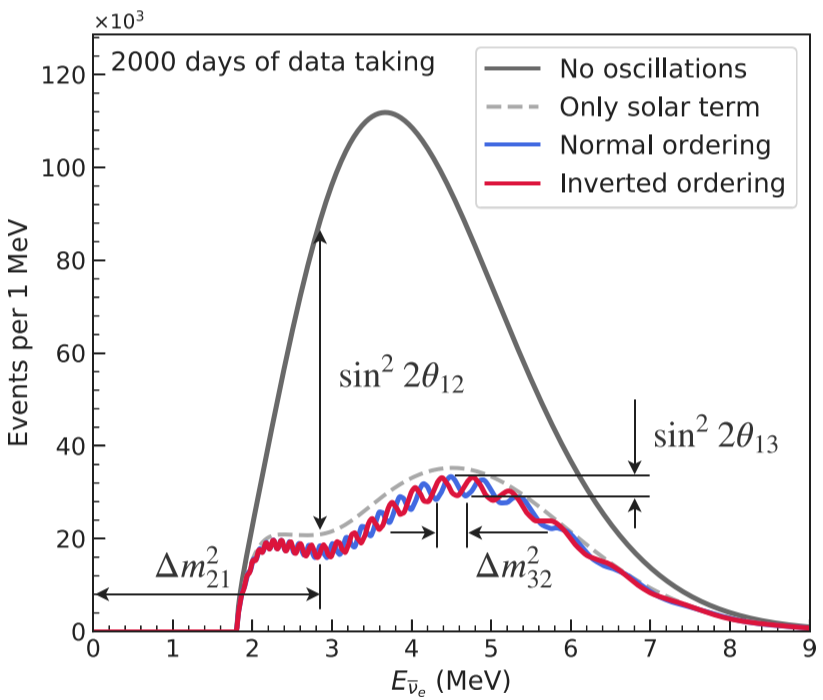
\includegraphics[width=0.4\linewidth]{Images/antineutino_to_antineutrino_probability_plot}
	\caption{JUNO's reactor antineutrino energy spectrum is shown with and without the effect of neutrino oscillation. The gray dashed curve includes only the term in the disappearance probability modulated by $sin^2(2\theta_{12})$, while the blue and red curves use the full oscillation probability for normal and inverted mass orderings. Spectral features driven by oscillation parameters are illustrated, highlighting the rich information available in JUNO's high-resolution measurement of the oscillated spectrum.}
	\label{fig:antineutinotoantineutrinoprobabilityplot}
\end{figure}


JUNO's primary objective is to refine these results, particularly to ascertain the sign of $\Delta m_{31}^2$, which will distinguish between two potential scenarios:
\begin{itemize}
	\item \textit{Normal Ordering (NO)}, where $\left|\Delta m_{31}^2\right|=\left|\Delta m_{32}^2\right|+\left|\Delta m_{21}^2\right|$ and the mass hierarchy is $m_1<m_2<m_3$,
	\item \textit{Inverted Ordering (IO)}, where $\left|\Delta m_{31}^2\right|=\left|\Delta m_{32}^2\right|-\left|\Delta m_{21}^2\right|$ and the mass hierarchy is $m_3<m_1<m_2$.
\end{itemize}
The sign of $\Delta m_{31}^2$ subtly alters the plot of \ref{fig:antineutinotoantineutrinoprobabilityplot}. However, it remains uncertain whether the $\nu_3$ neutrino mass eigenstate is heavier or lighter than the $\nu_1$ and $\nu_2$ mass eigenstates.


\section{The JUNO detector}

Nestled beneath the Dashi hill in Jinji town, Southern China, the Jiangmen Underground Neutrino Observatory (JUNO) is an ongoing experiment. Its placement 43 km southwest of Kaiping city was strategically chosen to significantly reduce background noise from cosmic rays due to its underground location. JUNO is anticipated to detect a plethora of antineutrinos, predominantly originating from the Taishan and Yangjiang nuclear power plants (NPPs). These power plants are approximately 52.5 km away from the JUNO detector and together, they have a combined nominal thermal power of 26.6 $GW_{th}$. The detector's design has been meticulously optimized for the highest sensitivity to the ordering of neutrino masses.\\

A schematic illustration of JUNO is presented in Fig.\ref{fig:junoschemeexperiment}.


\begin{figure}[h]
	\centering
	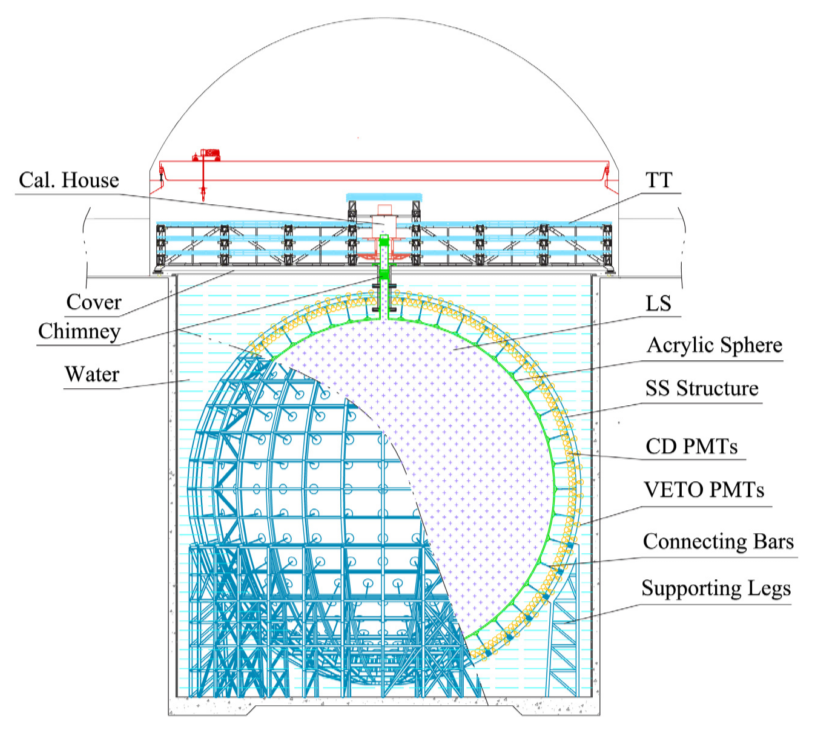
\includegraphics[width=0.6\linewidth]{Images/juno_scheme_experiment}
	\caption[JUNO scheme experiment]{Schematic view of the JUNO experiment}
	\label{fig:junoschemeexperiment}
\end{figure}


Furthermore, the JUNO experiment deploys a specialized compact detector named TAO. Situated approximately 30 meters from one of the Taishan reactors, TAO serves to measure the unoscillated reactor antineutrino spectrum shape precisely. The data collected by TAO is intended to provide a crucial data-driven input to refine the spectra from the other reactor cores. \\
The core of the JUNO detector, the \textbf{Central Detector (CD)}, is complemented by a water \textbf{Cherenkov detector} and a \textbf{Top Tracker (TT)}. Notably, the CD, designed as a compact, non-segmented detector, boasts an effective energy resolution of $\sigma_E/E =3\% / \sqrt{E (MeV)}$, a testament to the advantage of opting for a compact design over a segmented one.\\

The CD contains a 20 kton liquid scintillator (LS), safely housed within a spherical acrylic vessel and submerged in a water pool. The pool, with a diameter of 43.5 m and a height of 44 m, provides an adequate buffer to shield the LS from the radioactive influence of the surrounding rock.

The vessel is supported by a stainless steel (SS) structure through connecting bars. Additional CD PMTs are mounted on the inner surface of this structure, which also hosts compensation coils designed to mitigate the Earth's magnetic field and thereby minimize its impact on the photoelectron collection efficiency of the PMTs.

Above the water pool resides the Top Tracker, an assembly of a plastic scintillator array, meticulously arranged to measure muon tracks accurately. The CD is connected to the external environment through a chimney, which facilitates calibration operations. Located above this chimney is the Calibration House, equipped with special radioactivity shielding and a muon detector, playing a crucial role in the overall experimental setup.

\newpage

\section{JUNO signal and background}

\subsection{Signal}
%TODO: Aggiungere REACTOR FLUX sul unoscill file
%LIQUID SCINTILLATOR

The JUNO experiment primarily draws its sources from the Taishan and Yangjiang Nuclear Power Plants (NPPs), which house two and six cores respectively. In addition to these, the Daya Bay reactor complex contributes to the antineutrino flux. The reactor power, baselines, and anticipated Inverse Beta Decay (IBD) rates from the Taishan, Yangjiang, and Daya Bay reactor cores are detailed in Table \ref{tab:IBD_reactor_source}.


\begin{table}[htp]
	\centering
	\begin{tabular}{|c|c|c|c|}
		\hline
		Reactor & Power [$GW_{th}$] & Baseline [Km]  & IBD Rate [$day^{-1}$] \\\hline\hline
		Taishan & 9.2 & 52.71 &	15.1	\\\hline
		Yangjiang & 17.4 & 52.46 & 29.0	\\\hline
		Daya Bay & 17.4 & 215 &	3\\\hline
	\end{tabular}
	\caption{Information on nuclear reactors}
	\label{tab:IBD_reactor_source}
\end{table}


JUNO employs a Liquid Scintillator (LS) primarily composed of Linear Alkyl-Benzene (LAB), known for its transparency, high flash points, robust light yield, and low chemical reactivity. The LS, with a density of 0.859 $g/mL$, is further enhanced with 3 $g/L$ of 2,5-diphenyloxazole (PPO) as the fluor, and 15 $mg/L$ of p-bis-(o-methylstyryl)-benzene (bis-MSB) as the wavelength shifter. The scintillator is doped with a small amount of gadolinium, increasing its sensitivity to antineutrinos via the inverse beta decay (IBD) process.\\

This process is initiated when an antineutrino interacts with a proton in the liquid scintillator, producing a positron and a neutron. It can be described by the following reaction:

\begin{equation}
	\begin{aligned}
		\overline{\nu}_e + p &\rightarrow e^+ + n \\
	\end{aligned}
\end{equation} 
IBD is characterized by a comparatively low threshold of 1.8 MeV, a substantial cross section, and it can be readily differentiated from the background due to its delayed $\gamma$ signature.\\

The positron, carrying the majority of the antineutrino's initial energy, deposits this energy in the scintillator through ionization. This energy deposition, coupled with the positron's subsequent annihilation typically into two 0.511 MeV photons, forms the prompt signal, characterized as follow: $e^{+} + e^{-} \rightarrow 2\gamma$.
The energy deposited by the positron directly correlates with the antineutrino energy, providing a precise measure critical for neutrino oscillation studies.\\

Following the prompt signal, the neutron is captured primarily on hydrogen (approximately 99$\%$ of the time) after an average delay of about 220 µs. This capture event releases a single 2.2 MeV photon, creating the delayed signal. Occasionally, the neutron is captured on carbon (around 1$\%$ of the time), resulting in a gamma-ray signal with a total energy of 4.9 MeV. The process is described as follows:

\begin{equation}
	 n + ^{1}\text{H} \rightarrow ^{2}\text{H}^{*} \rightarrow ^2\text{H} + \gamma
\end{equation}
 
Despite carrying only a small fraction of the initial antineutrino energy, typically from zero to a few tens of keV, neutron recoils are considered in the calculations due to JUNO's exceptional energy resolution.

The light output from these events is detected by the photomultiplier tubes (PMTs), sensitive detectors that convert light into an electrical signal. They operate based on the photoelectric effect and subsequent electron multiplication. The signals from all the PMTs are then combined to reconstruct the position and energy of the original neutrino interaction. This technique allows JUNO to measure the energy of the incoming neutrino to high precision, which is crucial for studying neutrino oscillation. %When a photon hits the photocathode (the light-sensitive surface inside the PMT), it can eject an electron through the photoelectric effect. This electron is then accelerated by an electric field towards a series of electrodes called dynodes. Each time an electron hits a dynode, more electrons are released. This process is repeated multiple times, resulting in a cascade of electrons and a significant amplification of the original signal. The final electrical signal, which can be easily measured, is proportional to the number of photons that hit the photocathode. 

\newpage 

\subsection{Background}
The design and composition of the scintillator in the JUNO experiment are meticulously optimized to minimize background noise from various radiation sources, such as cosmic rays and natural radioactivity. Despite these efforts, several types of background signals are inevitably produced in the detector. For the purpose of analysis, we focus primarily on the three most significant contributors:


\subsubsection*{Radiogenic Backgrounds}


Radiogenic backgrounds in the JUNO experiment primarily originate from the radioactive decay of isotopes such as $^{238}\mathrm{U}$, $^{232}\mathrm{Th}$, and $^{40}\mathrm{K}$. These isotopes are naturally present in the materials comprising the JUNO detector, including acrylic used for the detector walls, the metal structure supporting the detector, PMT glass, the gas during early filling phases, and the surrounding water. They are also found in the surrounding rock. These isotopes undergo radioactive decay, emitting various forms of radiation. The decay of $^{238}\mathrm{U}$ and $^{232}\mathrm{Th}$ occurs through decay chains, where each isotope successively decays into different isotopes, releasing radiation in the process. The emitted radiation includes alpha particles, beta particles, and gamma rays. As for $^{40}\mathrm{K}$, it undergoes beta decay to $^{40}\mathrm{Ca}$ or electron capture to $^{40}\mathrm{Ar}$, with a small fraction (0.001$\%$) resulting in the emission of a gamma ray. These radiogenic backgrounds need to be carefully accounted for and minimized to accurately detect reactor antineutrinos in the JUNO experiment.


These radiogenic backgrounds can potentially mimic the signal from inverse beta decay (IBD) in several ways:

\begin{enumerate}
%TODO: Aggiungii range energetici, così puoi spiegare più o meno l'andamento delle energie 
	\item \textbf{Beta decays and electron captures}: These processes result in the emission of electrons or positrons, which can produce a scintillation signal similar to the prompt signal from IBD.

	\item \textbf{Gamma rays}: High-energy gamma rays can Compton scatter in the detector, producing electrons with enough energy to mimic the prompt signal from IBD. In addition, gamma rays can produce electron-positron pairs in the detector, which can mimic both the prompt and delayed signals from IBD.
	
	\item \textbf{Neutrons}: Some decays in the $^{238}\mathrm{U}$ and $^{232}\mathrm{Th}$ chains emit neutrons, which can be captured on protons in the detector, mimicking the delayed signal from IBD.

\end{enumerate}

\subsection*{Cosmogenic Backgrounds}

Cosmogenic backgrounds in JUNO primarily result from the interaction of cosmic rays, particularly high-energy muons ($\mathcal{O}(\text{GeV})$), with the detector materials. These interactions lead to the production of fast neutrons and unstable isotopes through the process of spallation in which a high-energy particle strikes a target atom, causing it to emit smaller particles such as neutrons and unstable isotopes. Specifically, these muons interact with the detector materials, resulting in the production of isotopes like  $^{9}\mathrm{Li}$, $^{8}\mathrm{He}$ and $^{11}\mathrm{C}$, which are unstable and subsequently decay, contributing to additional background events.

These fast neutrons and unstable isotopes, produced from the interactions of muons with the detector materials, can generate signals that mimic an inverse beta decay (IBD) event. Specifically, there are two distinct signals to consider.

The first, known as the prompt signal, is generated by an electron. The energy and momentum of this electron can make it appear like a positron, the particle that would be expected in an IBD event. The second, known as the delayed signal, is generated by a neutron. This neutron can be captured by a proton in the detector, producing a signal identical to what would be expected from the neutron in an IBD event.\\

Therefore, even though they are not IBD events, these signals mimic an IBD event as they consist of an electron being mistaken for a positron in the prompt signal and a true neutron in the delayed signal.



\subsubsection*{Other source of  $\overline{\nu}_e$}

Other sources of antineutrinos also contribute to the background. Those are geoneutrinos, atmospheric neutrinos, and reactor antineutrinos:\\

\textbf{Geoneutrinos} are antineutrinos produced by natural radioactivity within the Earth, primarily below 2.5 MeV in antineutrino energy. Natural radioactivity exists in materials present in the Earth's crust and mantle, such as $\mathrm{U}$, $\mathrm{Th}$,and $^{40}\mathrm{K}$. These materials undergo radioactive decays, generating antineutrinos as decay products, that produce IBD signals.\\

\textbf{Atmospheric neutrinos} are generated by interactions of cosmic rays with the Earth's atmosphere. When high-energy cosmic rays collide with the atmosphere, they produce a cascade of particles, including muons and neutrinos. The muons generated in these interactions can decay, producing antineutrinos.\\

\textbf{Reactor antineutrinos} are an artificial source of antineutrinos. Besides the reactors that are used to generate the signal to be analyzed, there are various other reactors that contribute to the total event count. Given the vast number of nuclear reactors worldwide, the collective signal from these reactors becomes significant.\\


%TODO: aggiungi perchè i neutrini solari non sono sorgente di BKG (?)


It's beneficial to categorize the aforementioned background sources into two distinct groups:

\begin{itemize}
	\item \textit{Accidental Background}: This category includes background events that result from the coincidence of two independent events, typically of radiogenic origin. These events primarily influence the low-energy region of the spectrum. A portion of the cosmogenic background also falls into this category. The goal of this thesis work is to significantly reduce these accidental background events, a topic that will be discussed in detail in the following sections
	\item \textit{Correlated Backgrounds}: These backgrounds originate from a single physics process and produce both a prompt and a delayed signal. Significant correlated backgrounds include cosmogenic Li/He and fast neutrons. Among all the radiogenic processes, only one correlated background requires consideration: the $\mathrm{C}$($\alpha$,n)$^{16}\mathrm{O}$, decay that produces an alpha particle (prompt signal) and a neutron that is captured as delayed, exactly like an IBD, occurring within the liquid scintillator.
\end{itemize}
 





Here a viasualization sumary of all the bacgrounds contributions:

\begin{figure}[h]
	\centering
	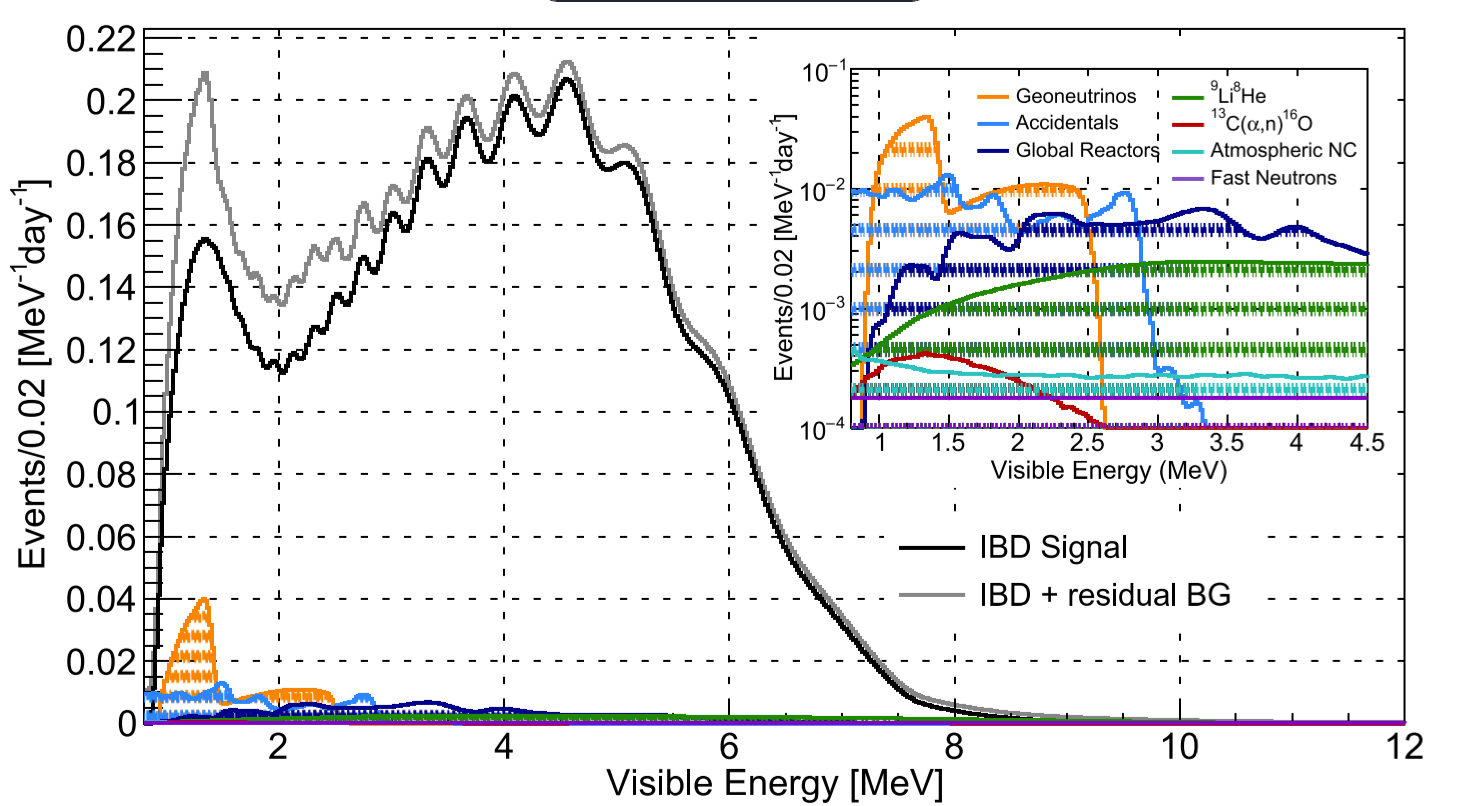
\includegraphics[width=0.7\linewidth]{Images/backgrounds_spectrum}
	\caption{Visible energy spectrum with (grey) and without (black) backgrounds is that which is anticipated for JUNO. The predicted backgrounds, which make up around 7$\%$ of the whole sample of IBD candidates and are primarily confined below, are shown in the inset as spectra. $\approx$ 3 MeV}
	\label{fig:backgroundsspectrum}
\end{figure}


Following the comprehensive discussion of all background events in the JUNO experiment, it becomes clear that due to the significant presence of various types of background events, efforts are being made to reduce their contribution in every possible way. Several strategies have been employed to mitigate these background signals. Methods include the use of shielding materials to block external radiation, careful selection and treatment of detector materials to minimize internal radioactivity, and sophisticated data analysis techniques to identify and reject background events.

However, it's important to note that a large portion of the accidental background events are the only ones where significant reduction can be achieved. These are the events that occur randomly and independently, and their reduction requires a different approach compared to correlated backgrounds. The focus of this thesis is precisely on these accidental background events, exploring strategies and techniques to further minimize their impact on the experiment.\\
This is a crucial aspect of the experiment's success, as reducing these events can significantly improve the sensitivity and accuracy of the neutrino measurements.	 
